% Compile:
%   pdflatex deepfm_report.tex
% or:
%   latexmk -pdf deepfm_report.tex
%
% Notes:
% - This document focuses on Model 4: DeepFM.
% - For an overall comparison across all models, see `REPORT.md` and `report.tex`.
% - For interactive plots with one-click PNG/SVG downloads, open `plots/report_graphs.html`.

\documentclass[11pt]{article}

\usepackage[margin=1in]{geometry}
\usepackage{microtype}
\usepackage{amsmath}
\usepackage{booktabs}
\usepackage{graphicx}
\usepackage{siunitx}
\usepackage{enumitem}
\usepackage{xcolor}
\usepackage{hyperref}
\usepackage{pgfplots}
\usepackage{pgfplotstable}
\usepackage{subcaption}
\usepackage{longtable}
\usepackage{tabularx}
\usepackage{array}
\usepackage{listings}

\pgfplotsset{compat=1.18}
\sisetup{detect-weight=true, detect-family=true}
\hypersetup{
  colorlinks=true,
  linkcolor=blue!60!black,
  urlcolor=blue!60!black,
  citecolor=blue!60!black
}

\lstset{
  basicstyle=\ttfamily\small,
  breaklines=true,
  columns=fullflexible,
  frame=single,
  framerule=0.3pt,
  rulecolor=\color{black!20},
  upquote=true
}

\usetikzlibrary{positioning,arrows.meta,shapes.geometric}

% -----------------------------
% Key numbers (copied from this repo's tensors/results as of 2026-03-12)
% -----------------------------
\newcommand{\NTotal}{597{,}928}
\newcommand{\NTrain}{418{,}549}
\newcommand{\NVal}{89{,}689}
\newcommand{\NTest}{89{,}690}

% Robustness: eval_suite (full features)
\newcommand{\AnnRandRmseMean}{0.1420}
\newcommand{\AnnRandRmseStd}{0.0036}
\newcommand{\AnnRandAccMean}{92.64}
\newcommand{\AnnRandAccStd}{0.31}

\newcommand{\HedRandRmseMean}{0.2446}
\newcommand{\HedRandRmseStd}{0.0030}
\newcommand{\HedRandAccMean}{87.76}
\newcommand{\HedRandAccStd}{0.10}

\newcommand{\AnnTimeRmseMean}{0.3146}
\newcommand{\AnnTimeRmseStd}{0.0365}
\newcommand{\AnnTimeAccMean}{82.78}
\newcommand{\AnnTimeAccStd}{2.35}

\newcommand{\HedTimeRmseMean}{0.5947}
\newcommand{\HedTimeRmseStd}{0.0162}
\newcommand{\HedTimeAccMean}{69.35}
\newcommand{\HedTimeAccStd}{1.09}

% DeepFM full-train (3 seeds: 0/1/42)
\newcommand{\DeepRandRmseMean}{0.1708}
\newcommand{\DeepRandRmseStd}{0.0085}
\newcommand{\DeepRandAccMean}{91.22}
\newcommand{\DeepRandAccStd}{0.51}

\newcommand{\DeepTimeRmseMean}{0.3533}
\newcommand{\DeepTimeRmseStd}{0.0107}
\newcommand{\DeepTimeAccMean}{75.74}
\newcommand{\DeepTimeAccStd}{1.51}

% Best DeepFM full-train run (from results_all.csv)
\newcommand{\BestDeepfmRunName}{\texttt{deepfm\_best\_fulltrain\_seed1}}
\newcommand{\BestDeepfmTestRmse}{0.1621}
\newcommand{\BestDeepfmTestAcc}{91.80}
\newcommand{\BestDeepfmNParams}{3{,}146{,}151}

% Best DeepFM sweep run (50k cap; from results_all.csv)
\newcommand{\BestDeepfmSweepName}{\texttt{deepfm\_huge\_k16\_hd2048-1024-512\_d0.05}}
\newcommand{\BestDeepfmSweepTestRmse}{0.2851}
\newcommand{\BestDeepfmSweepTestAcc}{89.70}

% Illustrative DeepFM run (trained in this environment; 50k train cap, seed=42)
\newcommand{\IllBestEpoch}{39}
\newcommand{\IllBestTestRmse}{0.2768}
\newcommand{\IllBestTestAcc}{89.52}
\newcommand{\IllLastTestRmse}{0.2812}
\newcommand{\IllLastTestAcc}{89.07}

% -----------------------------
% Inline data tables used by pgfplots (illustrative DeepFM run; train_max=50k)
% -----------------------------

\pgfplotstableread[col sep=space]{
epoch trainrmse valrmse valacc
1 6.949910 3.838429 0.000000
2 2.550029 2.233188 22.303188
3 1.628233 1.654352 19.217896
4 1.121439 1.142703 60.538208
5 0.799998 0.927855 70.249304
6 0.616376 0.769556 78.964378
7 0.515965 0.699145 83.057763
8 0.468591 0.658117 84.707797
9 0.443770 0.638382 85.945927
10 0.430783 0.616987 86.359932
11 0.418903 0.602014 86.951262
12 0.410672 0.590003 87.302536
13 0.405813 0.579621 87.322752
14 0.401480 0.568993 87.332311
15 0.397906 0.556103 87.759542
16 0.394111 0.548512 87.865718
17 0.388339 0.529968 87.671614
18 0.389958 0.528322 87.897576
19 0.380625 0.511856 88.270207
20 0.377033 0.505844 88.051102
21 0.373223 0.500011 88.622514
22 0.375297 0.493514 88.339770
23 0.369155 0.487870 87.610797
24 0.366701 0.477448 88.615506
25 0.364522 0.466800 88.431709
26 0.361010 0.458644 89.012525
27 0.356839 0.468968 85.040067
28 0.361289 0.450000 88.359044
29 0.353901 0.453378 86.218441
30 0.356317 0.435245 88.964140
31 0.351694 0.428906 88.487859
32 0.350009 0.422698 88.107891
33 0.345430 0.418234 89.107943
34 0.345333 0.414856 88.876960
35 0.347026 0.407728 89.266353
36 0.344985 0.408404 88.673601
37 0.343302 0.410931 86.269718
38 0.347649 0.397298 88.175631
39 0.337944 0.385956 89.635666
40 0.344418 0.388528 89.118338
}\DeepFMCurve

\pgfplotstableread[col sep=space]{
center count
-0.975 25
-0.925 33
-0.875 38
-0.825 57
-0.775 61
-0.725 95
-0.675 136
-0.625 187
-0.575 272
-0.525 362
-0.475 535
-0.425 734
-0.375 983
-0.325 1475
-0.275 2083
-0.225 3206
-0.175 4799
-0.125 7159
-0.075 9365
-0.025 11346
0.025 11812
0.075 10676
0.125 8361
0.175 5903
0.225 3694
0.275 2219
0.325 1330
0.375 887
0.425 543
0.475 322
0.525 236
0.575 140
0.625 89
0.675 77
0.725 49
0.775 31
0.825 34
0.875 32
0.925 31
0.975 15
}\DeepFMResidHist

\pgfplotstableread[col sep=space]{
true pred
13.474429 13.549570
12.861001 12.813833
15.228447 15.681711
13.746161 13.514386
12.694655 12.686073
13.426167 13.335476
12.945628 12.784007
12.535380 12.652987
14.187075 14.482804
12.989977 13.013046
13.656516 13.576588
14.607598 14.445443
13.244583 12.802621
13.190023 13.207968
13.099710 13.250360
12.506181 12.669172
13.178745 12.990531
13.343907 13.244152
12.358798 12.627186
12.771389 12.728754
13.180634 13.276323
13.415034 13.156496
13.712925 13.509574
13.668751 13.464558
12.691584 12.716036
13.444448 13.411188
14.220976 14.392248
12.528160 12.501607
13.475835 13.320801
12.644331 12.218565
13.361382 13.346174
14.138319 14.164108
13.127353 13.134666
13.514407 13.534426
13.361382 13.399705
12.884109 13.091558
13.407544 13.138856
13.737550 13.928225
12.861001 13.061801
13.296318 13.369143
12.951577 12.905941
13.586099 13.434072
13.060490 13.235119
13.635188 13.370602
13.171155 13.185362
13.537780 13.456505
14.316286 14.127354
13.235694 13.259901
13.681980 14.276772
13.269059 13.340110
13.820499 13.911119
14.731802 13.811988
13.180634 13.279089
13.380876 12.899410
14.038655 13.986120
13.366096 12.887079
12.827995 12.642792
12.943000 13.142899
12.560248 12.579115
12.785213 12.673991
12.366920 12.317483
11.938200 11.843617
13.549630 13.489203
13.981026 14.116653
13.487008 13.453020
13.051407 12.827828
13.132316 13.183895
12.971542 13.379492
14.039454 14.224787
13.384729 13.445200
13.089636 13.151904
13.260386 13.069855
12.611541 13.105068
12.923915 12.886194
13.302685 13.177512
13.338283 13.141815
14.054528 14.212914
12.362226 12.238132
13.393155 13.415052
13.055157 13.117451
13.337477 13.134996
13.038984 13.073666
13.369225 13.452456
12.230770 12.324378
13.556741 13.717101
13.132316 13.043910
13.315626 13.285327
13.441545 13.445787
12.542548 12.418612
12.570719 12.532333
13.849913 13.721461
12.470362 12.314406
13.536987 13.262904
14.014362 13.668871
12.796636 12.662896
14.040653 13.936542
13.381647 13.722283
13.610945 13.525485
13.353477 13.219936
13.422469 13.523438
12.542548 12.839279
14.445719 14.298823
13.715692 13.779220
13.623140 13.569869
12.911398 12.885365
12.577640 12.641664
12.988834 12.934734
11.571204 11.835250
12.873648 13.193579
13.081544 12.999515
14.046623 13.610660
12.873648 12.753272
13.233907 12.882546
12.765692 12.866282
13.279368 13.111158
12.663184 12.865508
13.784021 13.648299
14.004891 13.651652
13.226726 13.135328
13.785052 13.888406
}\DeepFMPredScatter

\pgfplotstableread[col sep=space]{
year acc mdape n
2010 89.584970 10.415030 7414
2011 89.632380 10.367620 8798
2012 89.957998 10.042002 8855
2013 89.668214 10.331786 8339
2014 89.826120 10.173880 9755
2015 89.677540 10.322460 10545
2016 89.346678 10.653322 11446
2017 88.783347 11.216653 10194
2018 90.229800 9.770200 7279
2019 88.869417 11.130583 4251
}\DeepFMByYear

\pgfplotstableread[col sep=space]{
decile acc mdape n lo hi
1 90.501896 9.498104 8959 308.0 816.0
2 88.506664 11.493336 8316 816.0 1050.0
3 88.908311 11.091689 8543 1050.0 1200.0
4 89.091405 10.908595 9430 1200.0 1350.0
5 89.809281 10.190719 9314 1350.0 1550.0
6 90.080522 9.919478 6859 1550.0 1714.3
7 89.568220 10.431780 11242 1714.3 1950.0
8 89.930705 10.069295 8891 1950.0 2300.0
9 90.339561 9.660439 9161 2300.0 2836.0
10 88.141191 11.858809 8975 2836.0 14850.0
}\DeepFMByAreaDecile

% -----------------------------
% DeepFM sweep summaries (full features, random split, train_max=50k)
% -----------------------------
\pgfplotstableread[col sep=space]{
center count
0.275 5
0.325 23
0.375 38
0.425 38
0.475 26
0.525 25
0.575 10
0.625 11
0.675 7
0.725 4
0.775 6
0.825 2
0.875 0
0.925 2
0.975 1
1.025 0
1.075 2
}\DeepFMSweepRmseHist

\pgfplotstableread[col sep=space]{
rmse acc
0.433412 86.946233
0.519878 81.462297
0.385162 85.479139
0.460005 87.729663
0.510257 75.977634
0.346864 87.888814
0.537741 85.521479
0.618261 85.834064
0.614405 85.076928
0.470302 87.048523
0.518386 87.811372
0.380562 88.260642
0.550226 86.345156
0.348796 87.696198
0.382585 88.435688
0.544125 88.573440
0.304950 86.993994
0.331851 88.444041
0.714347 82.799217
0.383781 86.302917
0.356923 86.656277
0.374112 85.251622
0.394339 88.313651
0.445489 86.303586
0.410810 86.414210
0.959093 78.876047
0.543572 80.119041
0.497281 79.560131
0.367210 88.407343
0.575353 83.394757
0.387845 86.725117
0.514847 85.618076
0.781977 62.225890
0.503481 83.523950
0.303242 88.055046
0.299443 88.807574
0.449964 86.286949
0.388643 87.381844
0.408591 86.859284
0.607250 87.751331
0.295464 88.580360
0.444569 82.129373
0.531086 81.528342
0.607546 80.534200
0.404822 85.478674
0.473371 86.342897
0.346135 87.418009
0.318590 88.122173
0.540630 85.599636
0.403563 87.983374
0.450798 87.292100
0.560051 82.483825
0.473132 89.403357
0.428551 87.201150
0.754716 83.881296
0.661377 76.198608
0.533257 85.714009
0.399417 88.383078
0.532380 85.922335
0.524894 86.913730
0.807031 71.006227
0.399763 85.042228
0.388815 88.160472
0.325440 88.560157
0.451094 86.291094
0.434498 84.324850
0.459665 83.600576
0.455750 85.589172
0.322611 88.390582
0.906030 45.346493
0.444913 86.538158
0.391501 86.215064
0.367273 88.232993
0.301350 87.592038
0.393204 86.491649
0.328274 89.549956
0.694916 81.086764
0.602505 74.616730
0.319594 88.240872
1.077135 64.342692
0.491862 86.029917
0.712510 80.251220
0.460223 85.161389
0.376225 87.637593
0.508765 83.726037
0.598788 84.752926
0.454753 86.773002
0.430715 82.916473
0.509662 85.208718
0.346487 87.816710
0.329586 88.485222
0.466342 83.281916
0.698450 85.892078
0.526700 86.112280
0.344725 88.133934
0.410076 87.106057
0.362437 87.191999
0.623795 79.572664
0.371454 87.858099
0.323459 87.962567
0.503151 85.937245
0.606133 87.085244
0.393682 87.792590
0.551588 69.101712
0.461502 86.797754
0.354873 87.742547
0.516079 82.938065
0.416093 86.663024
0.665735 82.133865
0.483318 84.555811
0.384161 86.667639
0.334765 86.925732
0.742300 63.103771
0.355668 87.848072
0.547852 74.831352
0.402589 88.647147
0.285064 89.704178
0.907320 81.238157
0.358147 87.360305
0.486554 82.422504
}\DeepFMSweepScatter

\pgfplotstableread[col sep=space]{
valacc testacc
86.991763 86.946233
81.561579 81.462297
85.554427 85.479139
87.769584 87.729663
75.898519 75.977634
88.025251 87.888814
85.561353 85.521479
86.004120 85.834064
85.133152 85.076928
87.085229 87.048523
87.946970 87.811372
88.356662 88.260642
86.433212 86.345156
87.767177 87.696198
88.542278 88.435688
88.658010 88.573440
87.016103 86.993994
88.551230 88.444041
82.802474 82.799217
86.382668 86.302917
86.758441 86.656277
85.294455 85.251622
88.380130 88.313651
86.382324 86.303586
86.530295 86.414210
78.856443 78.876047
80.040963 80.119041
79.569685 79.560131
88.514786 88.407343
83.528461 83.394757
86.888947 86.725117
85.668783 85.618076
62.246242 62.225890
83.582585 83.523950
88.086434 88.055046
88.801224 88.807574
86.410974 86.286949
87.551465 87.381844
86.923571 86.859284
87.741064 87.751331
88.653824 88.580360
82.071002 82.129373
81.600870 81.528342
80.718358 80.534200
85.613273 85.478674
86.417803 86.342897
87.511714 87.418009
88.089740 88.122173
85.735813 85.599636
88.069562 87.983374
87.452069 87.292100
82.553075 82.483825
89.462537 89.403357
87.273633 87.201150
83.895651 83.881296
76.237850 76.198608
85.659392 85.714009
88.467228 88.383078
85.933514 85.922335
87.006436 86.913730
71.094865 71.006227
85.076986 85.042228
88.294132 88.160472
88.585876 88.560157
86.384681 86.291094
84.450628 84.324850
83.713515 83.600576
85.656248 85.589172
88.364469 88.390582
45.381033 45.346493
86.645594 86.538158
86.268644 86.215064
88.294683 88.232993
87.655053 87.592038
86.543258 86.491649
89.549027 89.549956
81.134060 81.086764
74.830610 74.616730
88.180756 88.240872
64.413166 64.342692
86.050943 86.029917
80.135104 80.251220
85.294530 85.161389
87.691768 87.637593
83.893901 83.726037
84.796898 84.752926
86.823229 86.773002
83.046520 82.916473
85.359885 85.208718
87.918644 87.816710
88.506722 88.485222
83.394779 83.281916
86.057566 85.892078
86.194271 86.112280
88.154400 88.133934
87.235922 87.106057
87.279864 87.191999
79.581068 79.572664
87.948449 87.858099
87.953155 87.962567
86.051077 85.937245
87.171786 87.085244
87.899318 87.792590
69.069257 69.101712
86.966185 86.797754
87.809743 87.742547
83.034953 82.938065
86.699834 86.663024
82.332973 82.133865
84.740615 84.555811
86.683936 86.667639
86.933285 86.925732
63.137302 63.103771
87.956791 87.848072
74.836308 74.831352
88.702384 88.647147
89.750310 89.704178
81.432267 81.238157
87.431231 87.360305
82.506861 82.422504
}\DeepFMSweepValTestAcc

\title{DeepFM (FM + MLP)\\
\large Architecture, Results, and Analysis}
\author{RPSAps360 Project}
\date{March 12, 2026}

\begin{document}
\maketitle

\begin{abstract}
This document explains the \textbf{DeepFM} tabular model implemented in this repo (\texttt{train\_deepfm.py}), summarizes its best results on the housing transaction dataset, and provides a set of professional report-ready figures (seed sensitivity, sweep distributions, learning curves, residual plots, subgroup performance, and interpretability views). All experiment rows are consolidated in a single canonical results sheet (\texttt{results\_all.csv}).
\end{abstract}

\tableofcontents
\newpage

\section{What DeepFM is (and why we use it)}
DeepFM is designed for tabular problems where both \textbf{(i) low-order feature interactions} and \textbf{(ii) nonlinear effects} matter. In housing, price depends on interactions such as size \(\times\) neighborhood, year \(\times\) location (market trends), and style \(\times\) city. DeepFM combines three components:
\begin{itemize}[leftmargin=*]
  \item a \textbf{linear} (wide) part, similar in spirit to hedonic regression,
  \item a \textbf{factorization-machine} interaction term capturing pairwise interactions efficiently,
  \item a \textbf{deep MLP} that models nonlinearities using learned embeddings.
\end{itemize}

\section{Model structure (math + diagram)}
\subsection{Mathematical form}
We predict \(y=\log(1+\text{price})\). DeepFM outputs:
\[
  \hat{y} =
  b
  + \underbrace{w^\top x_{\text{num}} + \sum_j w^{(j)}_{\text{cat}}[x_{\text{cat},j}]}_{\text{linear part}}
  + \underbrace{\frac{1}{2}\sum_{f=1}^k\left(\left(\sum_i v_{i,f}\right)^2 - \sum_i v_{i,f}^2\right)}_{\text{FM interactions}}
  + \underbrace{\text{MLP}([x_{\text{num}}, \text{flatten}(v_{\text{cat}})])}_{\text{deep part}},
\]
where \(k=\texttt{factor\_dim}\), numeric features use learned factor vectors scaled by their standardized value, and categorical features use embedding lookups.

\subsection{Architecture diagram}
\begin{figure}[h]
\centering
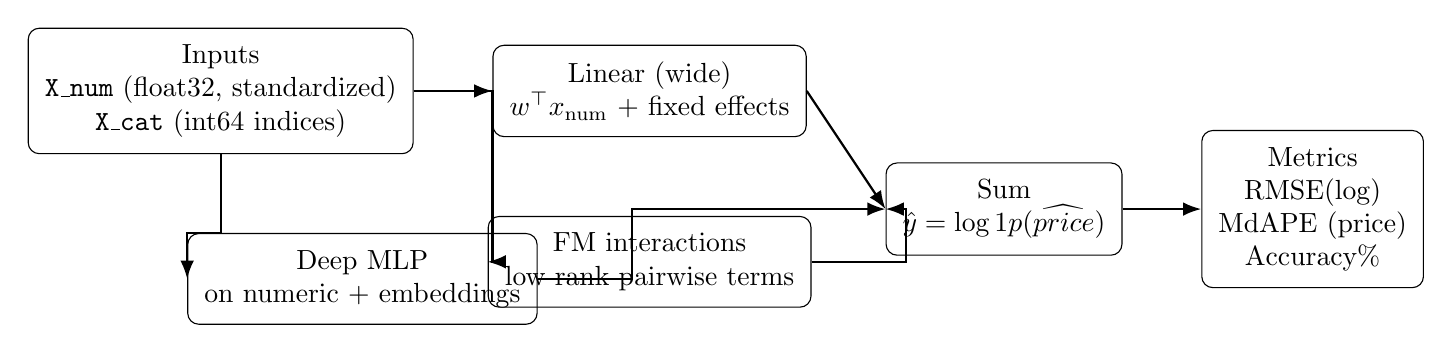
\begin{tikzpicture}[
  node distance=10mm,
  box/.style={draw, rounded corners, align=center, inner sep=6pt},
  arrow/.style={-Latex, thick}
]
\node[box] (inp) {Inputs\\
\texttt{X\_num} (float32, standardized)\\
\texttt{X\_cat} (int64 indices)};
\node[box, right=of inp] (lin) {Linear (wide)\\
\(w^\top x_{\text{num}}\) + fixed effects};
\node[box, below=of lin] (fm) {FM interactions\\
low-rank pairwise terms};
\node[box, below=of inp, xshift=18mm] (deep) {Deep MLP\\
on numeric + embeddings};
\node[box, right=of lin, yshift=-15mm] (sum) {Sum\\
\(\hat{y}=\log1p(\widehat{price})\)};
\node[box, right=of sum] (met) {Metrics\\
RMSE(log)\\
MdAPE (price)\\
Accuracy\%};
\draw[arrow] (inp) -- (lin);
\draw[arrow] (inp.east) -- ++(10mm,0) |- (fm.west);
\draw[arrow] (inp.south) -- ++(0,-10mm) -| (deep.west);
\draw[arrow] (lin.east) -- (sum.west);
\draw[arrow] (fm.east) -- ++(12mm,0) |- (sum.west);
\draw[arrow] (deep.east) -- ++(12mm,0) |- (sum.west);
\draw[arrow] (sum) -- (met);
\end{tikzpicture}
\caption{DeepFM combines linear terms, FM interactions, and a deep MLP (implementation: \texttt{train\_deepfm.DeepFM}).}
\label{fig:deepfm-diagram}
\end{figure}

\section{Data and preprocessing (reproducible)}
All experiments use the same tensorization pipeline as the other models:
\begin{itemize}[leftmargin=*]
  \item Source cleaned CSV: \texttt{cleaned\_transaction\_gtha-2.csv} (kept local).
  \item Tensorization: \texttt{prepare\_ann\_tensors.py --feature-set full} \(\rightarrow\) \texttt{ann\_tensors\_full.pt}.
  \item Dataset size: \textbf{\NTotal} total; split 70/15/15 into \textbf{\NTrain}/\textbf{\NVal}/\textbf{\NTest}.
\end{itemize}

\section{Experimental setup and metrics}
\subsection{Splits}
\begin{itemize}[leftmargin=*]
  \item \textbf{Random split:} standard 70/15/15 random partition.
  \item \textbf{Time split:} sort by (\texttt{TransactionYear}, \texttt{Quarter}) and split by time to evaluate future generalization.
\end{itemize}

\subsection{Metrics}
\begin{itemize}[leftmargin=*]
  \item \textbf{RMSE(log):} RMSE in \(\log1p(\text{price})\) space (lower is better).
  \item \textbf{MdAPE:} median absolute percentage error in price space.
  \item \textbf{Accuracy\%:} \(\max(0,100\cdot(1-\text{MdAPE}))\).
\end{itemize}

\section{Results summary}
\subsection{Best full-train DeepFM configuration (full features)}
From \texttt{results\_all.csv}, the best full-train DeepFM run is:
\begin{itemize}[leftmargin=*]
  \item Run name: \BestDeepfmRunName
  \item Hyperparams: \texttt{factor\_dim=16}, \texttt{hidden\_dims=2048,1024,512}, \texttt{dropout=0.05}, \texttt{epochs=40}, \texttt{batch\_size=4096}, \texttt{lr=0.002}, \texttt{weight\_decay=0.001}
  \item Parameters: \textbf{\BestDeepfmNParams}
  \item Test RMSE(log): \textbf{\BestDeepfmTestRmse}
  \item Test accuracy: \textbf{\BestDeepfmTestAcc\%}
\end{itemize}

\subsection{DeepFM vs ANN vs Hedonic (mean $\pm$ std)}
\begin{figure}[h]
\centering
\begin{subfigure}{0.49\linewidth}
\centering
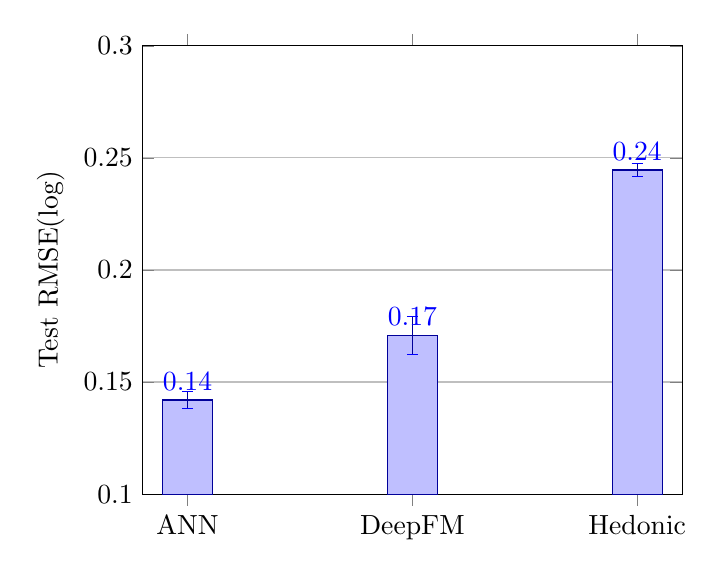
\begin{tikzpicture}
\begin{axis}[
  ybar,
  bar width=18pt,
  ylabel={Test RMSE(log)},
  symbolic x coords={ANN,DeepFM,Hedonic},
  xtick=data,
  ymin=0.10, ymax=0.30,
  ymajorgrids=true,
  error bars/y dir=both,
  error bars/y explicit,
  nodes near coords,
  nodes near coords align={vertical},
]
\addplot+[fill=blue!25, draw=blue!60!black] coordinates {
  (ANN,\AnnRandRmseMean) +- (0,\AnnRandRmseStd)
  (DeepFM,\DeepRandRmseMean) +- (0,\DeepRandRmseStd)
  (Hedonic,\HedRandRmseMean) +- (0,\HedRandRmseStd)
};
\end{axis}
\end{tikzpicture}
\caption{Random split RMSE(log).}
\end{subfigure}
\hfill
\begin{subfigure}{0.49\linewidth}
\centering
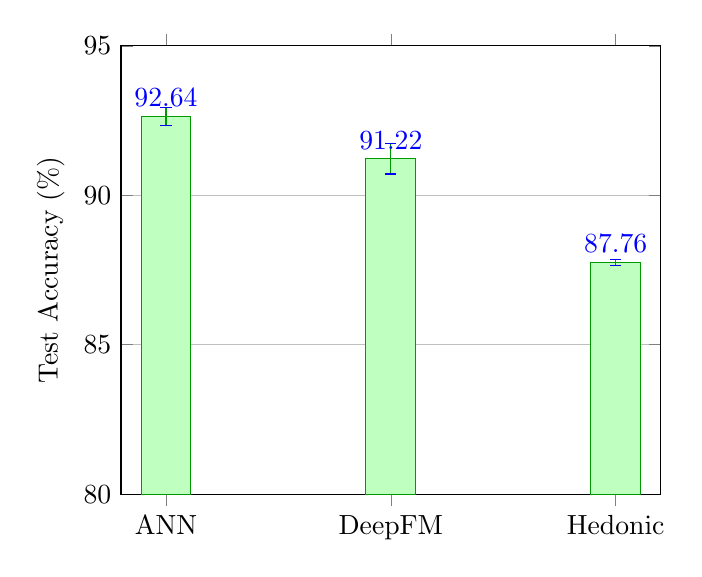
\begin{tikzpicture}
\begin{axis}[
  ybar,
  bar width=18pt,
  ylabel={Test Accuracy (\%)},
  symbolic x coords={ANN,DeepFM,Hedonic},
  xtick=data,
  ymin=80, ymax=95,
  ymajorgrids=true,
  error bars/y dir=both,
  error bars/y explicit,
  nodes near coords,
  nodes near coords align={vertical},
]
\addplot+[fill=green!25, draw=green!60!black] coordinates {
  (ANN,\AnnRandAccMean) +- (0,\AnnRandAccStd)
  (DeepFM,\DeepRandAccMean) +- (0,\DeepRandAccStd)
  (Hedonic,\HedRandAccMean) +- (0,\HedRandAccStd)
};
\end{axis}
\end{tikzpicture}
\caption{Random split accuracy.}
\end{subfigure}

\vspace{2mm}
\begin{subfigure}{0.49\linewidth}
\centering
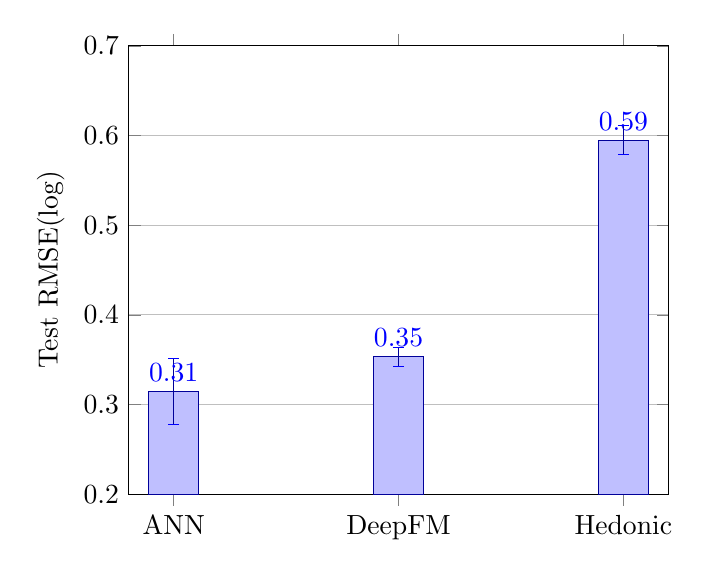
\begin{tikzpicture}
\begin{axis}[
  ybar,
  bar width=18pt,
  ylabel={Test RMSE(log)},
  symbolic x coords={ANN,DeepFM,Hedonic},
  xtick=data,
  ymin=0.20, ymax=0.70,
  ymajorgrids=true,
  error bars/y dir=both,
  error bars/y explicit,
  nodes near coords,
  nodes near coords align={vertical},
]
\addplot+[fill=blue!25, draw=blue!60!black] coordinates {
  (ANN,\AnnTimeRmseMean) +- (0,\AnnTimeRmseStd)
  (DeepFM,\DeepTimeRmseMean) +- (0,\DeepTimeRmseStd)
  (Hedonic,\HedTimeRmseMean) +- (0,\HedTimeRmseStd)
};
\end{axis}
\end{tikzpicture}
\caption{Time split RMSE(log).}
\end{subfigure}
\hfill
\begin{subfigure}{0.49\linewidth}
\centering
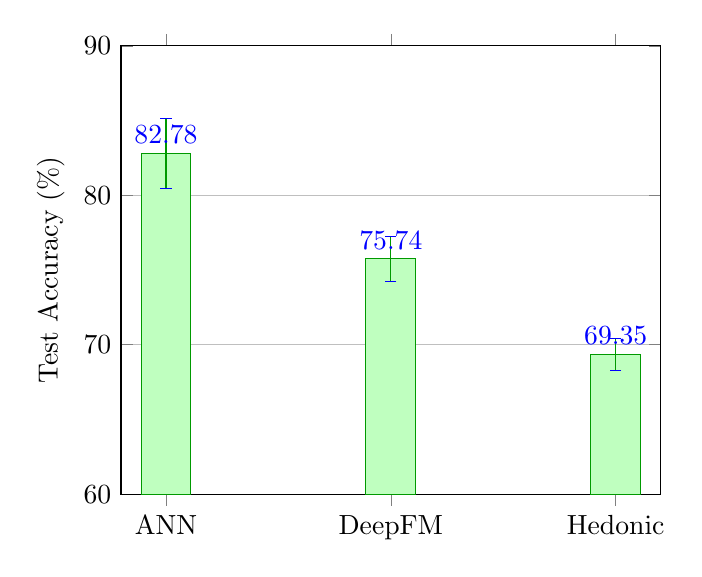
\begin{tikzpicture}
\begin{axis}[
  ybar,
  bar width=18pt,
  ylabel={Test Accuracy (\%)},
  symbolic x coords={ANN,DeepFM,Hedonic},
  xtick=data,
  ymin=60, ymax=90,
  ymajorgrids=true,
  error bars/y dir=both,
  error bars/y explicit,
  nodes near coords,
  nodes near coords align={vertical},
]
\addplot+[fill=green!25, draw=green!60!black] coordinates {
  (ANN,\AnnTimeAccMean) +- (0,\AnnTimeAccStd)
  (DeepFM,\DeepTimeAccMean) +- (0,\DeepTimeAccStd)
  (Hedonic,\HedTimeAccMean) +- (0,\HedTimeAccStd)
};
\end{axis}
\end{tikzpicture}
\caption{Time split accuracy.}
\end{subfigure}
\caption{DeepFM compared to ANN and hedonic baseline (mean $\pm$ std across seeds/splits as recorded in \texttt{results\_all.csv}).}
\label{fig:deepfm-compare}
\end{figure}

\subsection{Seed sensitivity (full-train DeepFM)}
\begin{figure}[h]
\centering
\begin{subfigure}{0.49\linewidth}
\centering
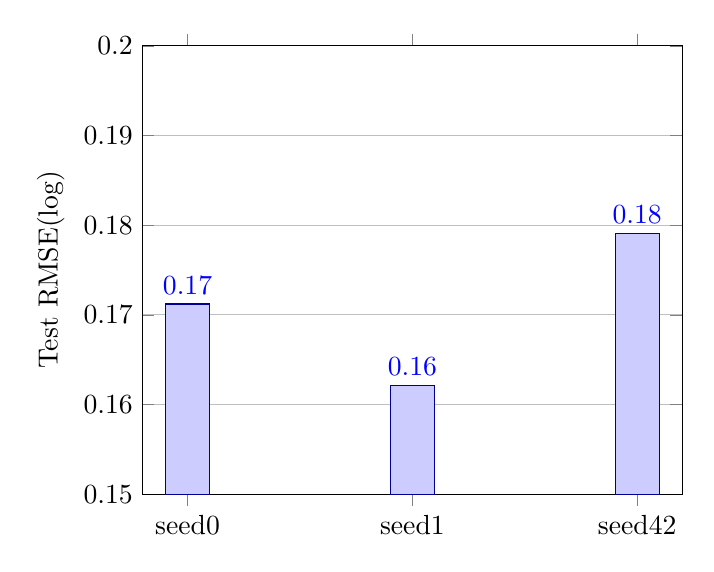
\begin{tikzpicture}
\begin{axis}[
  ybar,
  bar width=16pt,
  ylabel={Test RMSE(log)},
  symbolic x coords={seed0,seed1,seed42},
  xtick=data,
  ymin=0.15, ymax=0.20,
  ymajorgrids=true,
  nodes near coords,
  nodes near coords align={vertical},
]
\addplot+[fill=blue!20, draw=blue!60!black] coordinates {
  (seed0,0.1712)
  (seed1,0.1621)
  (seed42,0.1791)
};
\end{axis}
\end{tikzpicture}
\caption{Random split RMSE(log).}
\end{subfigure}
\hfill
\begin{subfigure}{0.49\linewidth}
\centering
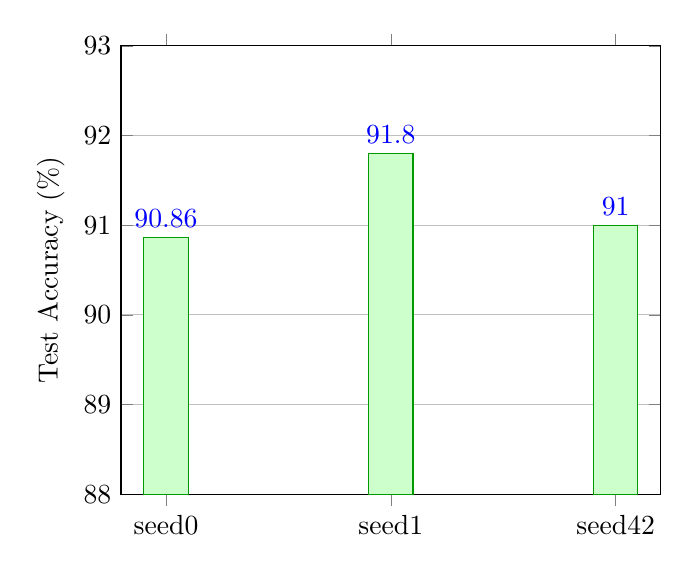
\begin{tikzpicture}
\begin{axis}[
  ybar,
  bar width=16pt,
  ylabel={Test Accuracy (\%)},
  symbolic x coords={seed0,seed1,seed42},
  xtick=data,
  ymin=88, ymax=93,
  ymajorgrids=true,
  nodes near coords,
  nodes near coords align={vertical},
]
\addplot+[fill=green!20, draw=green!60!black] coordinates {
  (seed0,90.86)
  (seed1,91.80)
  (seed42,91.00)
};
\end{axis}
\end{tikzpicture}
\caption{Random split accuracy.}
\end{subfigure}

\vspace{2mm}
\begin{subfigure}{0.49\linewidth}
\centering
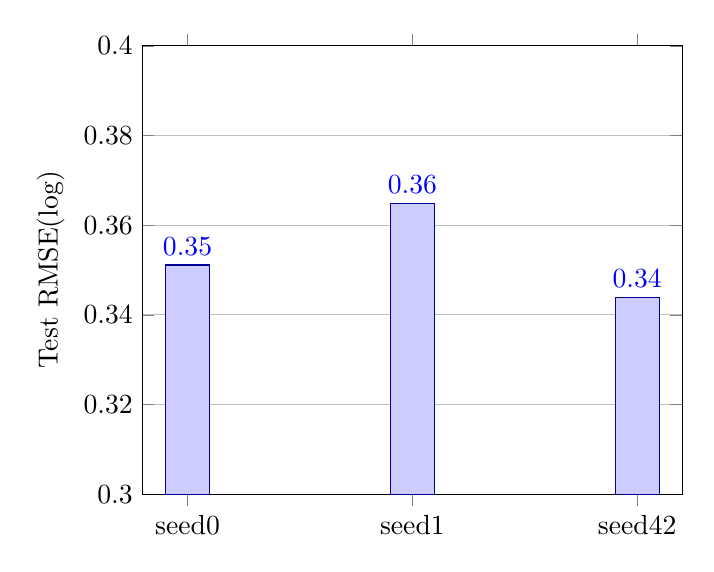
\begin{tikzpicture}
\begin{axis}[
  ybar,
  bar width=16pt,
  ylabel={Test RMSE(log)},
  symbolic x coords={seed0,seed1,seed42},
  xtick=data,
  ymin=0.30, ymax=0.40,
  ymajorgrids=true,
  nodes near coords,
  nodes near coords align={vertical},
]
\addplot+[fill=blue!20, draw=blue!60!black] coordinates {
  (seed0,0.3511)
  (seed1,0.3649)
  (seed42,0.3438)
};
\end{axis}
\end{tikzpicture}
\caption{Time split RMSE(log).}
\end{subfigure}
\hfill
\begin{subfigure}{0.49\linewidth}
\centering
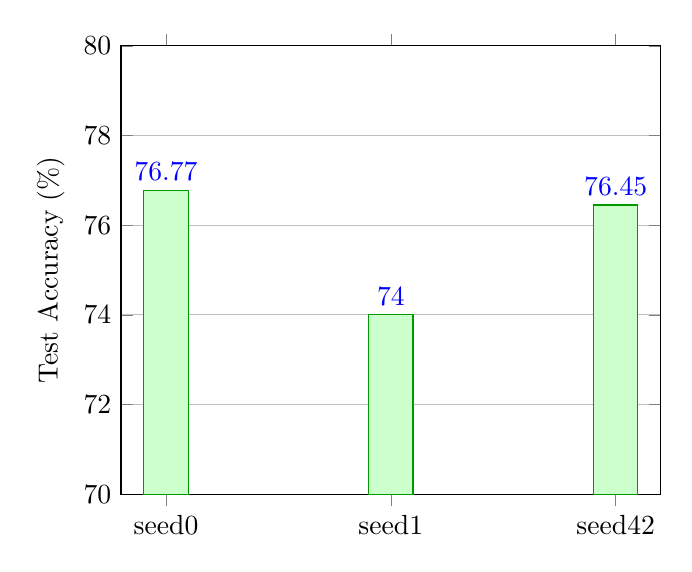
\begin{tikzpicture}
\begin{axis}[
  ybar,
  bar width=16pt,
  ylabel={Test Accuracy (\%)},
  symbolic x coords={seed0,seed1,seed42},
  xtick=data,
  ymin=70, ymax=80,
  ymajorgrids=true,
  nodes near coords,
  nodes near coords align={vertical},
]
\addplot+[fill=green!20, draw=green!60!black] coordinates {
  (seed0,76.77)
  (seed1,74.00)
  (seed42,76.45)
};
\end{axis}
\end{tikzpicture}
\caption{Time split accuracy.}
\end{subfigure}
\caption{DeepFM full-train performance across seeds (0/1/42) on random and time-based splits.}
\label{fig:deepfm-seeds}
\end{figure}

\section{Sweep results (many hyperparameter settings)}
\subsection{Best sweep configuration (50k train cap)}
From the 200-run randomized sweep (\texttt{sweep\_deepfm.py}; \texttt{train\_max\_samples=50,000}), the best configuration is:
\begin{itemize}[leftmargin=*]
  \item Name: \BestDeepfmSweepName
  \item Test RMSE(log): \textbf{\BestDeepfmSweepTestRmse}
  \item Test accuracy: \textbf{\BestDeepfmSweepTestAcc\%}
\end{itemize}

\subsection{Sweep distribution of test RMSE}
\begin{figure}[h]
\centering
\begin{tikzpicture}
\begin{axis}[
  ybar,
  bar width=8pt,
  xlabel={Test RMSE(log) bin center},
  ylabel={Count},
  xmin=0.25, xmax=1.10,
  ymajorgrids=true,
]
\addplot+[fill=blue!18, draw=blue!60!black] table[x=center,y=count] {\DeepFMSweepRmseHist};
\end{axis}
\end{tikzpicture}
\caption{Distribution of \texttt{test\_rmse} across 200 DeepFM sweep runs (full features, random split, 50k train cap).}
\label{fig:deepfm-sweep-hist}
\end{figure}

\subsection{Sweep trade-off: RMSE vs accuracy}
\begin{figure}[h]
\centering
\begin{tikzpicture}
\begin{axis}[
  xlabel={Test RMSE(log)},
  ylabel={Test Accuracy (\%)},
  xmin=0.25, xmax=1.10,
  ymin=40, ymax=92,
  grid=both,
]
\addplot+[only marks, mark=o, mark size=1.5pt, color=blue!60!black] table[x=rmse,y=acc] {\DeepFMSweepScatter};
\end{axis}
\end{tikzpicture}
\caption{Sweep trade-off scatter (each point = one DeepFM run).}
\label{fig:deepfm-sweep-scatter}
\end{figure}

\subsection{Validation vs test accuracy (sweep sanity check)}
\begin{figure}[h]
\centering
\begin{tikzpicture}
\begin{axis}[
  xlabel={Validation Accuracy (\%)},
  ylabel={Test Accuracy (\%)},
  xmin=40, xmax=92,
  ymin=40, ymax=92,
  grid=both,
  legend style={at={(0.02,0.98)},anchor=north west},
]
\addplot+[only marks, mark=triangle*, mark size=1.5pt, color=green!50!black] table[x=valacc,y=testacc] {\DeepFMSweepValTestAcc};
\addlegendentry{DeepFM sweep}
\addplot+[domain=40:92, samples=2, color=black!60] {x};
\addlegendentry{Ideal y=x}
\end{axis}
\end{tikzpicture}
\caption{Validation vs test accuracy for DeepFM sweep runs. Deviations from the diagonal indicate generalization gap or evaluation noise.}
\label{fig:deepfm-val-vs-test}
\end{figure}

\subsection{Overfitting frequency (sweep; RMSE-based)}
Because the best checkpoint is selected using validation MSE, a clean overfitting proxy is whether the last epoch has worse validation RMSE than the best checkpoint (\(\Delta = \texttt{val\_rmse\_last} - \texttt{val\_rmse}\)).

\begin{figure}[h]
\centering
\begin{tikzpicture}
\begin{axis}[
  ybar,
  bar width=26pt,
  xlabel={Overfitting bucket (Δval\_rmse)},
  ylabel={Count (out of 200)},
  symbolic x coords={0, (0,0.01], (0.01,0.05], >0.05},
  xtick=data,
  ymin=0, ymax=210,
  ymajorgrids=true,
  nodes near coords,
  nodes near coords align={vertical},
]
\addplot+[fill=orange!25, draw=orange!70!black] coordinates {
  (0,148)
  ((0,0.01],34)
  ((0.01,0.05],16)
  (>0.05,2)
};
\end{axis}
\end{tikzpicture}
\caption{Overfitting frequency across DeepFM sweep runs (full features, random split). Most runs hit their best validation RMSE at the final epoch (Δ=0).}
\label{fig:deepfm-overfit-buckets}
\end{figure}

\section{Training dynamics (illustrative run)}
To include learning curves and qualitative plots, we trained an illustrative DeepFM run in this environment with \texttt{train\_max\_samples=50,000} (val/test full), using the same hyperparameters as the best configuration found in sweeps. Best checkpoint results for this illustrative run:
\begin{itemize}[leftmargin=*]
  \item Best epoch: \textbf{\IllBestEpoch}
  \item Best-checkpoint test RMSE(log): \textbf{\IllBestTestRmse}, accuracy: \textbf{\IllBestTestAcc\%}
  \item Last-epoch test RMSE(log): \textbf{\IllLastTestRmse}, accuracy: \textbf{\IllLastTestAcc\%}
\end{itemize}

\begin{figure}[h]
\centering
\begin{subfigure}{0.49\linewidth}
\centering
\begin{tikzpicture}
\begin{axis}[
  xlabel={Epoch},
  ylabel={RMSE(log)},
  xmin=1, xmax=40,
  ymajorgrids=true,
  legend style={at={(0.02,0.98)},anchor=north west},
]
\addplot+[mark=*, mark size=1.1pt, color=blue!70!black] table[x=epoch,y=trainrmse] {\DeepFMCurve};
\addlegendentry{Train}
\addplot+[mark=triangle*, mark size=1.1pt, color=orange!80!black] table[x=epoch,y=valrmse] {\DeepFMCurve};
\addlegendentry{Validation}
\end{axis}
\end{tikzpicture}
\caption{RMSE(log) learning curve.}
\end{subfigure}
\hfill
\begin{subfigure}{0.49\linewidth}
\centering
\begin{tikzpicture}
\begin{axis}[
  xlabel={Epoch},
  ylabel={Validation Accuracy (\%)},
  xmin=1, xmax=40,
  ymin=0, ymax=92,
  ymajorgrids=true,
]
\addplot+[mark=*, mark size=1.1pt, color=green!60!black] table[x=epoch,y=valacc] {\DeepFMCurve};
\end{axis}
\end{tikzpicture}
\caption{Validation accuracy curve (MdAPE-derived).}
\end{subfigure}
\caption{Illustrative DeepFM learning curves (full features; 50k train cap).}
\label{fig:deepfm-curves}
\end{figure}

\section{Qualitative results (illustrative run)}
\subsection{Prediction scatter and residual distribution}
\begin{figure}[h]
\centering
\begin{subfigure}{0.49\linewidth}
\centering
\begin{tikzpicture}
\begin{axis}[
  xlabel={True log1p(price)},
  ylabel={Predicted log1p(price)},
  xmin=11.0, xmax=16.0,
  ymin=11.0, ymax=16.0,
  grid=both,
  legend style={at={(0.02,0.98)},anchor=north west},
]
\addplot+[only marks, mark=o, mark size=1.4pt, color=blue!60!black] table[x=true,y=pred] {\DeepFMPredScatter};
\addlegendentry{DeepFM (sample)}
\addplot+[domain=11:16, samples=2, color=black!60] {x};
\addlegendentry{Ideal y=x}
\end{axis}
\end{tikzpicture}
\caption{Predicted vs true (120 sampled test points).}
\end{subfigure}
\hfill
\begin{subfigure}{0.49\linewidth}
\centering
\begin{tikzpicture}
\begin{axis}[
  ybar,
  bar width=6pt,
  xlabel={Residual (pred\_log − true\_log)},
  ylabel={Count},
  xmin=-1.05, xmax=1.05,
  ymajorgrids=true,
]
\addplot+[fill=blue!18, draw=blue!60!black] table[x=center,y=count] {\DeepFMResidHist};
\end{axis}
\end{tikzpicture}
\caption{Residual histogram (test set).}
\end{subfigure}
\caption{Qualitative plots for DeepFM (illustrative run; best checkpoint).}
\label{fig:deepfm-qual}
\end{figure}

\subsection{Error by year and by property size}
\begin{figure}[h]
\centering
\begin{subfigure}{0.49\linewidth}
\centering
\begin{tikzpicture}
\begin{axis}[
  ybar,
  bar width=14pt,
  xlabel={TransactionYear (test subset)},
  ylabel={Accuracy (\%)},
  symbolic x coords={2010,2011,2012,2013,2014,2015,2016,2017,2018,2019},
  xtick=data,
  x tick label style={rotate=45,anchor=east},
  ymin=86, ymax=91,
  ymajorgrids=true,
]
\addplot+[fill=green!18, draw=green!60!black] table[x=year,y=acc] {\DeepFMByYear};
\end{axis}
\end{tikzpicture}
\caption{Accuracy by year.}
\end{subfigure}
\hfill
\begin{subfigure}{0.49\linewidth}
\centering
\begin{tikzpicture}
\begin{axis}[
  xlabel={LivingArea decile (1=smallest, 10=largest)},
  ylabel={Accuracy (\%)},
  xmin=1, xmax=10,
  ymin=86, ymax=91,
  grid=both,
  xtick={1,2,3,4,5,6,7,8,9,10},
]
\addplot+[mark=*, color=purple!60!black] table[x=decile,y=acc] {\DeepFMByAreaDecile};
\end{axis}
\end{tikzpicture}
\caption{Accuracy by LivingArea decile.}
\end{subfigure}
\caption{Subgroup performance diagnostics (illustrative run).}
\label{fig:deepfm-subgroups}
\end{figure}

\subsection{Selected examples (good/typical/hard)}
Table~\ref{tab:deepfm-examples} shows three representative test examples selected by absolute percentage error percentile (p5/p50/p95) for the illustrative run.

\begin{table}[h]
\centering
\small
\begin{tabularx}{\linewidth}{@{}lrrrrrll@{}}
\toprule
Example & True price & Pred price & APE (\%) & Year & LivingArea & FSA & City \\
\midrule
Good (p5) & 685{,}000 & 678{,}422 & 0.960 & 2016 & 2{,}275 & L6Y & BRAMPTON \\
Typical (p50) & 411{,}000 & 454{,}058 & 10.476 & 2015 & 1{,}550 & L6R & BRAMPTON \\
Hard (p95) & 1{,}291{,}000 & 784{,}380 & 39.242 & 2017 & 1{,}434 & M4R & TORONTO \\
\bottomrule
\end{tabularx}
\caption{Selected test samples for DeepFM (illustrative run).}
\label{tab:deepfm-examples}
\end{table}

\section{Interpretability (partial; linear components)}
DeepFM contains nonlinear components (FM interactions and deep MLP), so full interpretability is nontrivial. However, two easy-to-visualize components are:
\begin{itemize}[leftmargin=*]
  \item the \textbf{numeric linear weights} (\texttt{linear\_num}), and
  \item the \textbf{categorical linear fixed effects} (\texttt{linear\_cat}), which we center within a column for readability.
\end{itemize}

\begin{figure}[h]
\centering
\begin{subfigure}{0.49\linewidth}
\centering
\begin{tikzpicture}
\begin{axis}[
  xbar,
  xlabel={Coefficient (Δlog1p(price) per 1 std)},
  ytick=data,
  yticklabels={
    TransactionYear,
    gcode\_Lat,
    DistanceToSubj,
    LotSize,
    LivingArea,
    gcode\_Lon,
    KitchenCount,
    DOM,
    Bed\_Half,
    Bed\_Full,
    LandValue,
    Bath\_Full
  },
  ymin=-0.5, ymax=11.5,
  height=8cm,
  grid=both,
]
\addplot+[fill=blue!18, draw=blue!60!black] coordinates {
  (0.219213,0)
  (0.194184,1)
  (0.187358,2)
  (0.177676,3)
  (0.166475,4)
  (-0.165455,5)
  (0.161161,6)
  (0.151236,7)
  (0.132022,8)
  (-0.122460,9)
  (0.113536,10)
  (-0.061620,11)
};
\end{axis}
\end{tikzpicture}
\caption{Top numeric linear weights (illustrative run).}
\end{subfigure}
\hfill
\begin{subfigure}{0.49\linewidth}
\centering
\begin{tikzpicture}
\begin{axis}[
  ybar,
  bar width=12pt,
  ylabel={Centered fixed effect (Δlog1p(price))},
  symbolic x coords={M8X,L4X,L6J,M9R,L4Y,M4S,M5M,M4G,L1R,N3T,L1N,N1H,L4M,M5W,N0H,L0K},
  xtick=data,
  x tick label style={rotate=60,anchor=east},
  ymajorgrids=true,
]
\addplot+[fill=orange!22, draw=orange!70!black] coordinates {
  (M8X,0.021535)
  (L4X,0.017956)
  (L6J,0.016476)
  (M9R,0.015015)
  (L4Y,0.014894)
  (M4S,0.014873)
  (M5M,0.014581)
  (M4G,0.014194)
  (L1R,-0.031493)
  (N3T,-0.027834)
  (L1N,-0.027834)
  (N1H,-0.027834)
  (L4M,-0.027834)
  (M5W,-0.027834)
  (N0H,-0.027834)
  (L0K,-0.027834)
};
\end{axis}
\end{tikzpicture}
\caption{Centered FSA linear effects (examples).}
\end{subfigure}
\caption{Interpretability views for DeepFM (linear components only).}
\label{fig:deepfm-interpret}
\end{figure}

\section{Challenges and limitations (DeepFM-specific)}
\begin{itemize}[leftmargin=*]
  \item \textbf{Compute and tuning:} DeepFM has millions of parameters and multiple interacting components; it can underperform without careful learning-rate/regularization choices.
  \item \textbf{Distribution shift in time splits:} time-based evaluation is much harder; accuracy drops for all models, including DeepFM.
  \item \textbf{Interpretability:} FM + deep MLP components are not as directly interpretable as a pure hedonic regression. We use partial views (linear weights and centered fixed effects) plus error diagnostics.
\end{itemize}

\section{Plan for testing on never-before-seen data}
\begin{itemize}[leftmargin=*]
  \item \textbf{Preferred: fresh internal data.} Obtain a later transaction window not used during development (e.g.\ newer RPS exports) and evaluate the frozen DeepFM configuration once.
  \item \textbf{Fallback: external dataset.} If internal new data is not available, test on an entirely different public housing transaction dataset from a separate source/region.
\end{itemize}

\section*{Repro commands}
\begin{lstlisting}[language=bash]
# 1) Build full-feature tensors (from the cleaned CSV)
python prepare_ann_tensors.py --csv cleaned_transaction_gtha-2.csv \
  --out ann_tensors_full.pt --feature-set full

# 2) Train a DeepFM run (full train)
python train_deepfm.py --data ann_tensors_full.pt \
  --factor-dim 16 --hidden-dims 2048,1024,512 --dropout 0.05 \
  --epochs 40 --batch-size 4096 --lr 0.002 --weight-decay 0.001 \
  --seed 1 --run-name deepfm_best_fulltrain_seed1 --out-csv deepfm_runs.csv

# 3) Run a sweep (lots of configs; usually uses a 50k train cap for speed)
python sweep_deepfm.py --data ann_tensors_full.pt --n-runs 200 --resume

# 4) Merge everything into the single canonical results sheet
python export_results.py

# 5) Generate the offline HTML dashboard (with download buttons)
python make_report_graphs.py --results results_all.csv --out plots/report_graphs.html
\end{lstlisting}

\end{document}

